\documentclass[conference]{IEEEtran}
\IEEEoverridecommandlockouts
% The preceding line is only needed to identify funding in the first footnote. If that is unneeded, please comment it out.
\usepackage{cite}
\usepackage{amsmath,amssymb,amsfonts}
\usepackage{algorithmic}
\usepackage{graphicx}
\usepackage{textcomp}
\usepackage{xcolor}

\def\BibTeX{{\rm B\kern-.05em{\sc i\kern-.025em b}\kern-.08em
    T\kern-.1667em\lower.7ex\hbox{E}\kern-.125emX}}
\begin{document}

\title{CENG435 Term Project Part-1 Report\\}

\author{\IEEEauthorblockN{Simge Nur Çankaya}
\IEEEauthorblockA{\textit{Computer Engineering} \\
\textit{Middle East Technical University}\\
Ankara, Turkey \\
Student ID : 2099554 \\
Group ID : 36 \\
simgenurcankaya@gmail.com}
\and
\IEEEauthorblockN{Muhammed Süha Demirel}
\IEEEauthorblockA{\textit{Computer Engineering} \\
\textit{Middle East Technical University}\\
Ankara, Turkey \\
Student ID : 2098911 \\ 
Group ID : 36 \\
msuhademirel@gmail.com}
}

\maketitle

\begin{abstract}
In this project, we are expected to construct a network that consists of 5 nodes, which are connected to each other. The project is divided into two parts and this paper is written for the first part. In the first part; developing a UDP socket application, implementing a routing logic, sending message over UDP datagram and handling multiple request at the same time for all nodes are the main objectives. The scripts written for the nodes are tested on the virtual machines via GENI Platform. When the design and implementation are done, end-to-end delays are examined among the nodes. 
\end{abstract}

\begin{IEEEkeywords}
UDP, Node, IP, Port, Socket, Request, Routing Logic, End-to-End Delay
\end{IEEEkeywords}

\section{Specifications}
\begin{itemize}
    \item Developing a User Datagram Protocol(UDP) socket application.
    \item Only one script should run for each of the nodes.
    \item The scripts for each node should be executed once only.
    \item Each node should have a client/server application.
    \item Each node should receive and send messages.
    \item Each node should handle multiple requests. 
    \item An application-level routing logic will be used for the nodes.
\end{itemize}

\section{Introduction}
In the first part of the project, a slice has taken from the Global Environment for Network Innovations(GENI) platform and a unreliable virtual network, which consist 5 hosts, has established on the GENI. The hosts are :
\begin{itemize}
\item 1 source node
\item 3 router nodes
\item 1 destination node
\end{itemize}

UDP connection is implemented between these five nodes. Python's socket module and embedded scripts into the nodes are used in order to implement this configuration for the nodes. \\

1000 message packages to be sent between the nodes to find the costs of all links with round-trip time(RTT) and end-to-end delays between nodes. Then 3 experiments will be done with some delay additions to see the relation of network emulation delay and the end-to-end delay.

\section{Design \& Implementation}
The topology of a network is already given and its visual examination is shown Figure 1.

We used Kentucky Instageni Site to take slice and connect VMs. In order to connect VMs via ssh, we need to generate ssh keys(public and private keys). After the generation of keys, we need to add this key to our .ssh directory. Connection for a VM via ssh is established with the following code : \verb|ssh -i [SSH KEY_DIRECTORY]| \verb| e2099554@pc1.instageni.cs.kentucy.edu| \verb| -p [PORT_NUMBER]|. When the connection is established we are able to use our VM. To copy a file from our local machine to VM, we used the following code: \verb|scp -i [SSH KEY DIRECTORY] -P  [PORT_NUMBER]| \verb|[FILE DIRECTORY] e2099554@pc1.instageni.cs.| \verb|kentucy.edu:[COPY DIRECTORY]|.

We used GitHub for team communication and written our scripts with Python 2.

The topology of the network is imported to GENI Platform via .xml file. Also, we were given 2 configuration scripts named configureR1.sh and configureR2.sh to implement into node r1 and r2 via ssh. These scripts add random delays to determined links to the node that they run on.\\

\begin{figure}[h]
    \centering
    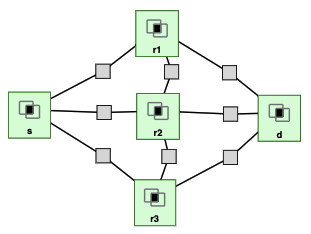
\includegraphics[width=8 cm, height=4 cm]{TheStructureOfTopology.png}
    \caption{The Structure of the Topology}
    \label{fig}
\end{figure}

Each node has unique Internet Protocol Address(IP address) for incoming and outgoing connections.  Embedded scripts into the nodes are used in order to implement UDP connection for the nodes. In these scripts, \verb|socket|, \verb|threading| and \verb|time| modules. Briefly explanation and some examples of the module usage for UDP ,which are taken from the project script, are given below.

For \verb|socket| module:
\begin{itemize}

    \item \verb|socket.socket(socket.AF_INET,|            \verb|  socket.SOCK_DGRAM)| : Socket function creates a new socket object.
        \begin{itemize}
        
        \item \verb|AF_INET| : A (host(IPv4), port(port)) pair is used for the \verb|AF_INET| address family. 
        
        \item \verb|SOCK_DGRAM| : The socket type for UDP. \\
        
        \end{itemize}
    
    \item \verb|socket.bind((IP_r1_d, PORT_r1))| : Bind the socket to address. The socket must not already be bound. \\

    \item \verb|socket.recvfrom(50)| : \verb|recvfrom()| Function receive data from the socket. The return value is a pair (bytes, address) where bytes is a bytes object representing the data received and address is the address of the socket sending the data. \\

\end{itemize}

For \verb|threading| module:
\begin{itemize}

    \item \verb|threading.Thread(target=sendS,| \verb| args=(ip_send_s,port_s))| : This is the constructor for thread and it should always be called with keyword arguments.
        \begin{itemize}
        \item \verb|target| : \verb|target| is the callable object to be invoked by the \verb|run()| method.
        
        \item \verb|args| : \verb|args| is the argument tuple for the target invocation. \\
        \end{itemize}
    
    \item \verb|thread.start()| : Starts the thread’s activity. It must be called at most once per thread object. It arranges for the object’s run() method to be invoked in a separate thread of control. \\
        
    \item \verb|thread.join(timeout=None)| : Waits until the thread terminates. This blocks the calling thread until the thread whose join() method is called terminates or until the optional timeout occurs. \\
    
\end{itemize}

For \verb|time| module:
\begin{itemize}

    \item \verb|time.time()| : Returns the time in seconds since the epoch as a floating point number. \\

    
\end{itemize}

As mentioned in Introduction part, each node has unique Internet Protocol Address(IP address) for incoming and outgoing connections. Moreover, the nodes need ports for sending packages to or receiving packages from other nodes. In the first version of the project, we thought that we need unique port numbers for each node for incoming and outgoing connections. However, we discovered that same port can be used for both receiving and sending.\\

The operator ports must be the same between two nodes, which are client and server(listener), in order to catch the packages. The port numbers have range from 0 to 65535, but only port numbers 0 to 1023 are reserved for privileged services and designated as well-known ports. Registered ports are 1024 to 49151. Dynamic ports (also called private ports) are 49152 to 65535. We have picked available port numbers in the range from 23426 to 45678.\\

The messages have been sent among the nodes have the string type and we are sending "Sent by R* ". To obtain more accurate results, 1000 messages, packages, have been sent from client nodes to server(listener) nodes.\\

Firstly, we focused on two specific nodes',r1 and r2, communication to understand the main logic. In the first step, we tried to send messages from r1 to r2, in another words, r1 was client and r2 was server. In the second step we changed the roles of the nodes; r1 became the server and r2 became the client. The next step was making both nodes client and server in the same time. This step has achieved but the a node was not able to handle receiving and sending packages in the same time. To solve this problem, we wrote down two different function for receiving and sending packages and implemented threads to nodes. Threading allows us to have different parts of your program run concurrently and can simplify our design. Therefore, a node is able to handle receiving and sending packages in the same time by using threads. For each node, r1 and r2, we used 1 receiver(server) thread and 1 sender(client) thread. Lastly, we implemented thread.join() function for each thread to make threads wait each other to terminate until end of the process. With the success of this two nodes concurrent communication, we move to the next step. \\

The next step we focused is concurrent communication of three nodes (r1, r2, s). We implemented the same scripts we wrote in the first part to the nodes. Different from the two nodes communication, nodes need to handle receive messages from 2 nodes and sending messages to 2 nodes.  Therefore, we implemented 2 receiver(server) threads and 2 sender(client) threads for each node.

The final step is achieving concurrent communication for all nodes according to the topology that is shown in Figure 1. And we implemented a routing table in a file which is named \verb|RoutingInformation.txt|.

We decided to use following logic to calculate and store the costs of the links: The costs of the links (s-r1, r1-r2, r1-d) are estimated and saved by r1, the costs of the links (s-r3, r2-r3, r3-d) are estimated and saved by r3, and finally, the costs of the links (s-r2, r2-d) are estimated and saved by r2. In order to make these calculations; r1 and r3 are set as client, s and d are set as server and r2 is set as both server and client. \\

When we examined our given topology on the GENI platform, we saw that the bandwidths of each link is like this:
\begin{itemize}
    \item r1$->$s and s$->$r1 : 1000 kbps
    \item r1$->$r2 and r2$->$r1 : 100 kbps
    \item r1$->$d and d$->$r1 : 1000 kbps
    \item r2$->$s and s$->$r2 : 1000 kbps
    \item r2$->$r3 and r3$->$r2 : 100 kbps
    \item r2$->$d and d$->$r2 : 1000 kbps
    \item s$->$r3 and r3$->$s : 2000 kbps
    \item r3$->$d and d$->$r3 : 2000 kbps
\end{itemize}.\\

We calculated RTTs between nodes with the following method: When we send the package from the client node to the server node, client node takes the time just before sending the package via time.time() then save it into a variable. When the server node receives the message package, it send the same package to the client node immediately (like acknowledgement package system). Just after the client receives the message back, it takes the current time again and saves it to another variable. The difference between these two time variable is our RTT. This method allows us to not to synchronize the different nodes' time because we always make time calculations according to the same node's time. RTT(link cost)s for each data transfer is stored like this:
\begin{itemize}
    
    \item RTTs are stored in node r1:
    \begin{itemize}
        \item between r1 and r2 for 1000 packages each RTT is stored in a .txt file named \verb|r1_r2.txt|.
        \item between r1 and s for 1000 packages each RTT is stored in a .txt file named \verb|r1_s.txt|.
        \item r1 and d for 1000 packages each RTT is stored in a .txt file named \verb|r1_d.txt|.
    \end{itemize}
    
    \item RTTs are stored in node r2:
    \begin{itemize}
        \item between r2 and s for 1000 packages each RTT is stored in a .txt file named \verb|r2_s.txt|.
        \item between r2 and d for 1000 packages each RTT is stored in a .txt file named \verb|r2_d.txt|.
    \end{itemize}
    
    \item RTTs are stored in node r3:
    \begin{itemize}
        \item between r3 and s for 1000 packages each RTT is stored in a .txt file named \verb|r3_s.txt|.
        \item between r3 and r2 for 1000 packages each RTT is stored in a .txt file named \verb|r3_r2.txt|.
        \item between r3 and d for 1000 packages each RTT is stored in a .txt file named \verb|r3_d.txt|.
    \end{itemize}
\end{itemize}

The average costs of the each link are stored in the nodes where RTTs are stored in files named \verb|avg.txt| and the average costs of the each link for 1000 packages is shown Figure 2.

\begin{figure}[h]
    \centering
    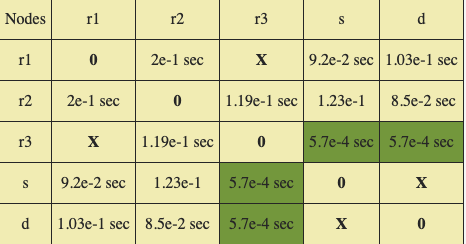
\includegraphics[width=8 cm, height=4 cm]{RTT-table.png}
    \caption{The Costs of the Links Between the Nodes}
    \label{fig}
\end{figure}

According to the table, the shortest path from node s(Source) to the node d(Destination) is like this: The node s must send packages to d via r3 [s $->$ r3 $->$ d]. \\

\section{Experimental Results}

In the project, we are expected to examine 3 experiment and to plot a figure that provides the relation of network emulation delay and the end-to-end delay with a 95\% confidence interval for each of the different communication. For each experiment, we added delays to links between node s - node r3 and node r3 - node d.

The experiments are listed below:
\begin{itemize}
    \item Default Configuration: There is no emulation delay.
    \item Experiment 1: Emulation delay is equal to $20ms\pm5ms$.
    \item Experiment 2: Emulation delay is equal to $40ms\pm5ms$.
    \item Experiment 3: Emulation delay is equal to $50ms\pm5ms$.

\end{itemize}.\\

To add emulation delay for the experiment 1 to the specified links, we used following codes derived from \verb|exp1.sh:|\\
\verb|sudo tc qdisc add dev $s_adapter root| \verb|netem delay 20ms 5ms distribution normal|.

\verb|sudo tc qdisc add dev $r2_adapter root| \verb|netem delay 20ms 5ms distribution normal|.

\verb|sudo tc qdisc add dev $d_adapter root| \verb|netem delay 20ms 5ms distribution normal|.

To add emulation delay for the experiment 2 to the specified links, we used following codes derived from \verb|exp2.sh:|\\
\verb|sudo tc qdisc change dev $s_adapter root| \verb|netem delay 40ms 5ms distribution normal|.

\verb|sudo tc qdisc change dev $r2_adapter root| \verb|netem delay 40ms 5ms distribution normal|.

\verb|sudo tc qdisc change dev $d_adapter root| \verb|netem delay 40ms 5ms distribution normal|.

To add emulation delay for the experiment 3 to the specified links, we used following codes derived from \verb|exp3.sh:|\\
\verb|sudo tc qdisc change dev $s_adapter root| \verb|netem delay 40ms 5ms distribution normal|.

\verb|sudo tc qdisc change dev $r2_adapter root| \verb|netem delay 40ms 5ms distribution normal|.

\verb|sudo tc qdisc change dev $d_adapter root| \verb|netem delay 40ms 5ms distribution normal|.\\

In the experiments, it is expected that sending 1 package from s to d via shortest path which is s$->$r3$->$d. But we sent 5 packages to be more accurate then took average of them. the results are shown below:
\begin{itemize}
    \item Result for default mode is 0.0035 (We sent only 1 package) 
    \item Result for experiment 1 is 0.0499 ± 0.00477: 
    \item Result for experiment 2 is 0.0852425 ± 0.00636:
    \item Result for experiment 3 is 0.103663 ± 0.00406:
\end{itemize}. \\

\begin{figure}[h]
    \centering
    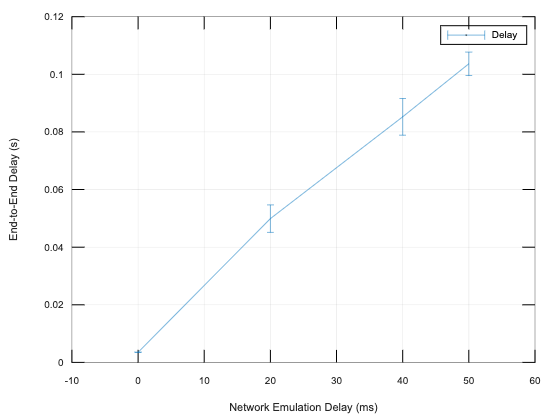
\includegraphics[width=8 cm, height=4 cm]{octave-online-line-10.png}
    \caption{The Relation of Network Emulation Delay and the End-to-End Delay }
    \label{fig}
\end{figure}

Deriving from the graph(Figure 3), we can say that emulation delay increased the end-to-end delay dramatically. 

\section{Conclusion}

With this project, we had a chance to discover how application layer looks like, what is a (partial) network, how UDP configuration can be implement, how end-to-end delay can be measured between nodes and how emulation delay can be added to the links between nodes. Also we experienced that if the the bandwidth increases, the RTT decrease and if emulation delay increases, the end-to-end delay increases.

\section*{References}
     threading - Thread-based parallelism¶. (n.d.). Retrieved from https://docs.python.org/3/library/threading.html. \\
    
     socket - Low-level networking interface¶. (n.d.). Retrieved from https://docs.python.org/3/library/socket.html. \\
    
     time - Time access and conversions¶. (n.d.). Retrieved from https://docs.python.org/3/library/time.html\#time.time. \\
     
     Page. (n.d.). Retrieved from https://wiki.python.org/moin/UdpCommunication. \\
     
     Updated November 02, 2017 / P. J. 24. (n.d.). List of Well-Known TCP Port Numbers. Retrieved from https://www.webopedia.com/quick\_ref/portnumbers.asp.


\end{document}

